% !TeX spellcheck = en_US
\section{Problem 6}

This problem depends on Problem 5, as it uses its technique to train a neural network.
The only thing changing here is the \verb|generate_AR_data()| function, that now creates a time series that is described using the following equation:
\[
X_t = U_t + a_1 U_{t-1} + a_2 U_{t-2} + a_3 U_{t-3} + a_4 U_{t-4} + a_5 U_{t-5} + a_6 U_{t-6}
\]
with $a_1 = a_2 = 5$ and $a_3 = a_4 = a_5 = a_6 = -0.5$.

\begin{minipage}{0.46\linewidth}
	\centering
	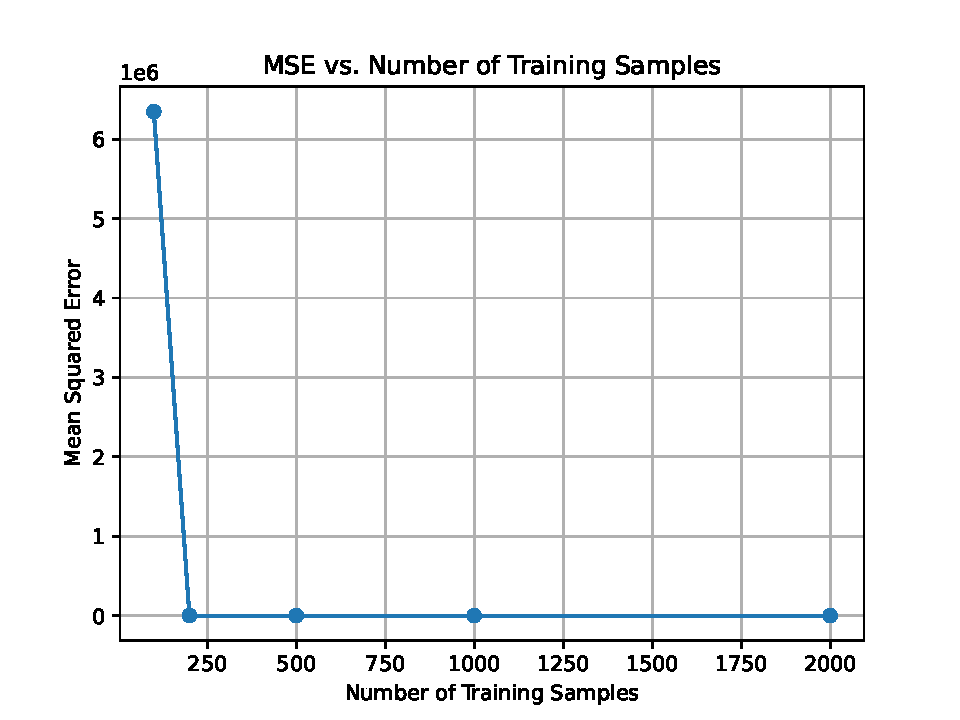
\includegraphics[width=0.8\linewidth]{../Problem 6/prob6_mse_vs_total_epoch.pdf}
	\captionof{figure}{Averaged cost square error function over number of training samples}
	\label{fig:prob6_mse_total_epoch}
\end{minipage} \hfill
\begin{minipage}{0.45\linewidth}
	\centering
	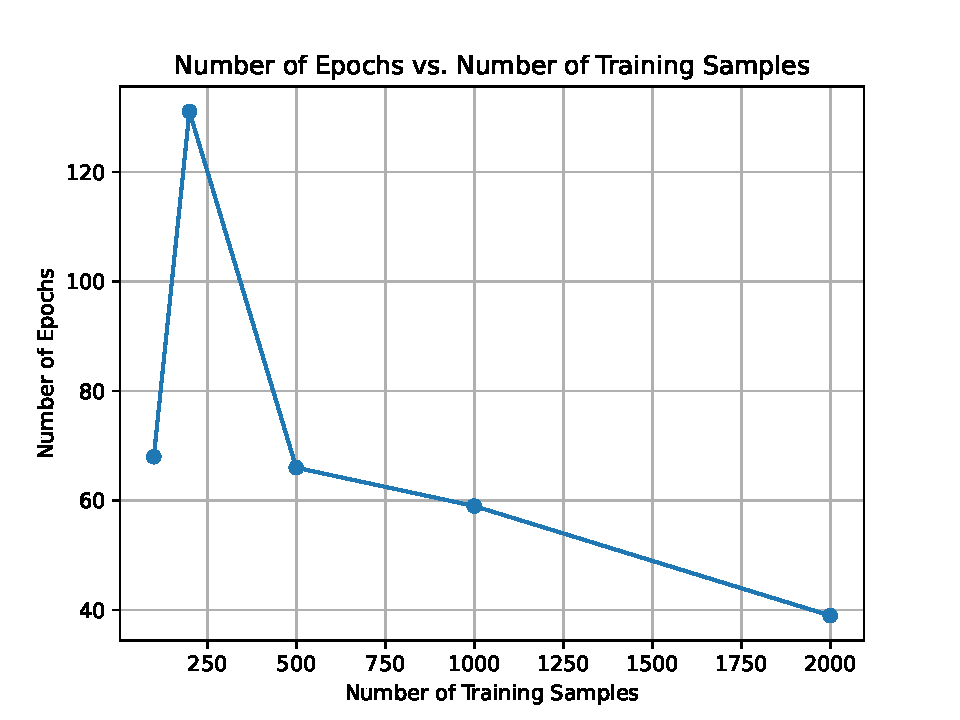
\includegraphics[width=0.8\linewidth]{../Problem 6/prob6_epoch_vs_training_samples.pdf}
	\captionof{figure}{Number of epochs required for the NN to converge}
	\label{fig:prob6_epoch_train_samples}
\end{minipage}
\\

Figures \ref{fig:prob6_mse_total_epoch} \& \ref{fig:prob6_epoch_train_samples} are generated with data taken from neural network's train procedure.\\

Both of these graphs together indicate a relationship between the amount of data the model is trained on and the model's performance and training characteristics. More data generally seems to lead to better performance (\textit{as seen by lower MSE}) and potentially more efficient training (\textit{fewer epochs needed as training samples increase}). The outlier or spike in the number of epochs at $200$ samples happened because NN's input was fairly small in size. 
If we look at even smaller values, we can see that the number of epochs is smaller than the one on $200$ samples but if we see the MSE number, we observe that network does anything than converging.

The $U_t$ being uniformly distributed means that it has a constant probability over the interval $(0, 0.5)$, and being independent and identically distributed means that each $U_t$ is drawn from the same distribution and is independent of others. The coefficients used for data generation suggest that $U_{t-1}$ and $U_{t-2}$ have a significant positive influence on the current value, while $U_{t-3}$ to $U_{t-6}$ have a small negative influence.\\

Overall, these graphs suggest that the LSTM model benefits from more data which is consistent with the behavior of most machine learning models, as LSTM are used for exactly this reason. 
\vspace{3mm}
